\documentclass{acm_proc_article-sp}
\usepackage{graphicx}
\usepackage{float}
\usepackage{url}
\makeatletter
\def\@copyrightspace{\relax}
\makeatother
\begin{document}


\setlength{\emergencystretch}{3em}

\title{I523: Project: 018: How Far have Cars driven the Nature!}

\subtitle{\url{https://gitlab.com/cloudmesh_fall2016/project-018/}}

\numberofauthors{2} 
\author{
% 1st. author
\alignauthor
Amruta Chavan\\
       \affaddr{MS in Data Science at}\\
       \affaddr{Indiana University of Bloomington}\\
       \affaddr{GitLab ID: amchavan}
       \email{amchavan@iu.edu}    
% 2nd. author
\alignauthor
Aditya Tanikanti\\
       \affaddr{MS in Data Science at}\\
       \affaddr{Indiana University of Bloomington}\\
       \affaddr{GitLab ID: aditya.tanikanti}
       \email{atanikan@iu.edu}      
}
\toappear{}
\maketitle

\begin{abstract}
This paper provides an insight into the fuel consumption and carbon emission by different car models driven all over the world. It analyses and compares performance of different types of cars based on types,brands and other specifications.

The project will throw light on how much and how badly are automobiles affecting the environment and causing Global Warming. It tries to find some fuel efficient cars and/or alternate solutions to avoid further damage to nature. Other important relationships and correlations between the various features will be explored through the built model.

\end{abstract}

\section{Introduction}
Global warming endangers our health, jeopardizes our national security, and threatens other basic human needs. Some impacts-such as record high temperatures, rising seas, and severe flooding and droughts-are already increasingly common.

Excessive amount of fuel consumption is causing runaway global climate change, threatening people, cities and ecosystems with a dangerous future of flooding,extreme heat, fires and super-storms. If the world can transition to renewable sources for almost all energy purposes within the next few decades. The sooner this is done, the sooner we will improve public health, build resilience and foster a clean-energy economy - and the less we will have to pay toward the high cost of climate adaptation.

Our personal vehicles are a major cause of global warming. Collectively, cars and trucks account for nearly one-fifth of all US emissions, emitting around 24 pounds of carbon dioxide and other global-warming gases for every gallon of gas. About five pounds comes from the extraction, production, and delivery of the fuel, while the great bulk of heat-trapping emissions-more than 19 pounds per gallon-comes right out of a car's tailpipe.

Unfortunately, oil-related emissions may rise in the coming years as the oil industry extracts and refines "unconventional" oils, such as tar sands and tight oil. Using less oil, avoiding unnecessary emission from the oil, finding alternative for fuel, cars etc, exploring various relationships between vehicle and its emissions over the years are few steps towards preventing global warming that this project will try to focus on. \cite{ConcernedScientists2014}


\section{Background}
In total, the US transportation sector-which includes cars, trucks, planes, trains, ships, and freight-produces nearly thirty percent of all US global warming emissions, more than almost any other sector. While in EU, cars are responsible for around 12 percent of total emissions of carbon dioxide ($CO_{2}$), the main greenhouse gas.

All new cars and light trucks sold in the U.S. are required to have a economy label posted on the window sticker. The label contains the city and highway miles-per-gallon values, as well as other related information. To calculate these values, laboratory tests are performed on pre-production vehicles.
This report will review and analyse the data to test and predict most efficiently performing vehicles that could reduce fuel emission.

The project tries to study the performance of various car models that have been launched since 1984-2017 and how their usage has been affecting environment.

\section{Data Sets}
This project uses data set published by US-EPA \textit{United States Environment Protection Agency}. Dataset links, can be found in the gitlab repository data folder or in the references as \cite{2014}, \cite{2015}.

\section{About the Data}
The vehicle data is collected and classified based on various test analysis and types such as drive type,type of fuel consumed,type of roads on which the car was driven and hence the fuel efficiency. It has 38032 rows or samples and 83 features also called as columns.

\section{Technologies}
We intend to use the following technologies in our project
\subsection{Python/Anaconda}
Python/Ipython Notebook(Anaconda) - For Data Cleaning/Wrangling, Exploratory Data Analysis and modeling data so as to predict $CO_{2}$ smog rating.

Download packages for python on anaconda by running requirements.txt

Optionally use PySpark to implement the modeling part in a map reduce format and to store the data in HDFS.\

Integrated pyspark for parallel processing however it's an optional feature. To download it properly in windows follow \cite{Kadamati2015}

\subsection{D3.js}
D3.js - Visualizing the graphs we generated via the exploratory data analysis phase.To get d3 visualizations to run in windows first run a command (based on the OS)
from a location where you download the files from code d3 files folder 

Use following html pages and the localhost port you're running on to get the code to run:\\
type\_emission\_per\_year.html, 
make\_emission.html

\section{Data Wrangling}
The dataset was processed and cleaned for futher analysis. The vehicle.csv and emission.csv datasets were consolidated into one single dataset for easier analysis based on the vehicle id column using Pyspark.
Two tables were created that summarize the data for data visualization based on the variables of concern namely fuel economy,annual fuel consumption and $CO_{2}$ emission etc.

\section{Descriptive Analysis and Data Trends}
The dataset was analysed to study 2 types of trends in the data set namely yearly variability in the data and Overall trend in the data set to derive conclusions.Yearly variability analysis deals with year-to-year of various factors leading to raise/drop in $CO_{2}$ Emission levels and Fuel Efficiency of the vehicles which may on may not be meaningful in long-term perspective. Overall Analysis deals will help to make definite correlations between factors causing depletion or augmentation of the harmful emissions by vehicles and propose solutions to thereby reduce the threat created to the environment through issues such Global Warming, Ozone Layer depletion, Glacier Melting etc.

Figure 1 and 2 shows $CO_{2}$ emissions and fuel economy for MY 1975-2016. The two plots essentially inversely proportional to each other, i.e., vehicle tailpipe $CO_{2}$ emissions (grams per mile) are proportional to fuel consumption (gallons per mile), which is the reciprocal of fuel economy (miles per gallon).
These two figures show that $CO_{2}$ emissions and fuel economy have undergone four clearly defined phases since 1975. Figure 2.3 shows fuel
economy, weight, and horsepower data for MY 1975-2016 from Table 2.1. All of the data in Figure 2.3 are presented as percentage changes since 1975. It's important to note, other things being equal, that vehicle weight and horsepower increases are generally associated with increased $CO_{2}$ emissions and decreased fuel economy. 

\section{Feature Selection and Predictive Modelling}

\subsection{Data Cleaning and Feature Extraction}
The data was sorted and we found the percentages of NULL, NA and -1(missing values) in the each column. The columns with NULL or NA or -1 percentage greater than 30$\%$ were removed from the data set. Upon cleaning the data, it's size reduced to 15 Features with approximately 26K Samples from original data set of 83 feature variables with 38K samples.

\subsection{Data Modelling}
The goal of doing predictive analysis was to build a model which will learn about the features of a clean or unclean vehicle (Smog Score of 1 to 10) with 10 being cleanest vehicle and 1 being the worst and then predict a smog score given features of a vehicle. To achieve this the data had to be modelled in such a way that it considers each of the 15 independent features perfectly.

Since the data was very sparse and there were categorical variables in features such as Make, Vehicle Type etc we first used Label Encoder in scikit learning package of python to convert all categorical variables into discrete values. We then scaled all the variables to fit into a range of 0 to 1 so as to help models perform better while predicting the class values.

Now the data was split into 80-20 train-test data with the class variable as Smog score which have a possibility of  and several algorithms were implemented in the project to evaluate the performance of each algorithm and choose best fit model for the data set.

Since it is a multiclass problem, 10 class variables to be precise, one needs to be aware of the limitations when it comes evaluating the models accuracy. 

Mentioned below are the different Machine Learning algorithms implemented on the data to obtain scores for the vehicles to test their performance and accuracy.

\subsubsection{Naive Bayes}
Naive Bayes classifier scales a number of parameters linear in the number of variables (features/predictors) in a learning problem. Upon implementation, Naive Bayes model gave accuracy of 45.81$\%$ and precision of 21$\%$ with F1 score of 29$\%$. \\

\begin{figure}[H]
\centering
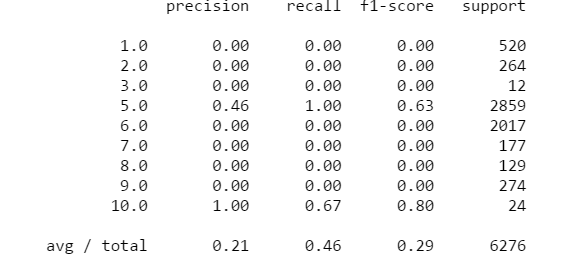
\includegraphics[height=2.5in, width=3.2in]{NB}
\caption{Multinomial Naive Bayes}
\end{figure}

\subsubsection{k-NN}
K-nearest neighbors is an algorithm that classifies new classes  based on a similarity measure along with the stored classes. 

\begin{figure}[H]
\centering
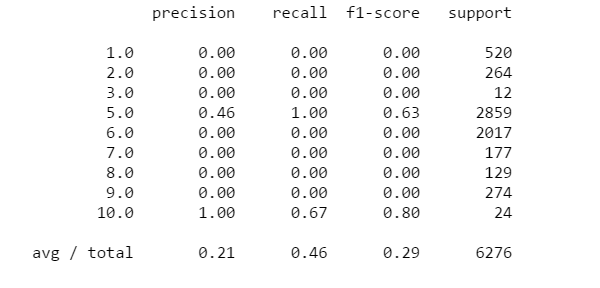
\includegraphics[height=2.5in, width=3.2in]{kNN}
\caption{k-Nearest Neighbours}
\end{figure}

The k-Nearest Neighbours algorithm gave accuracy of 41.70$\%$ and precision of 21$\%$ with F1 score of 29$\%$.

\subsubsection{Decision Tree}
A decision tree algorithm forms a tree-like structure with root node, branches, and leaf nodes where each internal node represents test preformed on an feature variable, each branch denotes the outcome of that test, and each leaf node holds a class label. 

\begin{figure}[H]
\centering
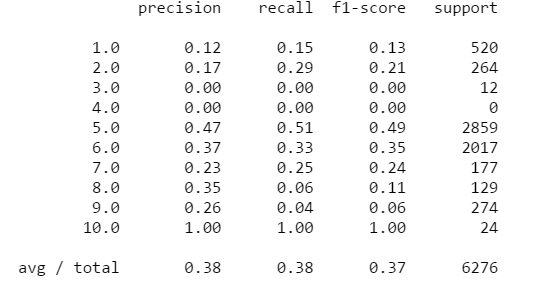
\includegraphics[height=2.5in, width=3.2in]{DecisionTree}
\caption{Decision Tree}
\end{figure}

Decision Tree implementation gave accuracy of 37.64$\%$ and precision of 38$\%$ with F1 score of 37$\%$. 

\subsubsection{SVC}
SVC is non-parametric clustering algorithm that classifies data based on boundaries implemented where the probability of occurance of data sample values is less irrespective of the feature variables.

\begin{figure}[H]
\centering
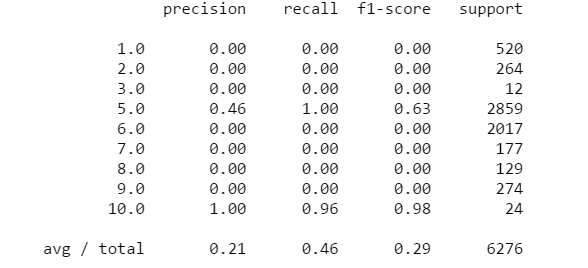
\includegraphics[height=2.5in, width=3.2in]{SVC}
\caption{Support Vector Clustering}
\end{figure}

Support Vector Clustering provides accuracy of accuracy of 45.92$\%$ and precision of 21$\%$ with F1 score of 29$\%$. 

\subsubsection{Random Forest}
Random Forest algorithm combines various classification techniques such as decision trees and regression models to extract best of all these methods for better accuracy and precision scores. 

\begin{figure}[H]
\centering
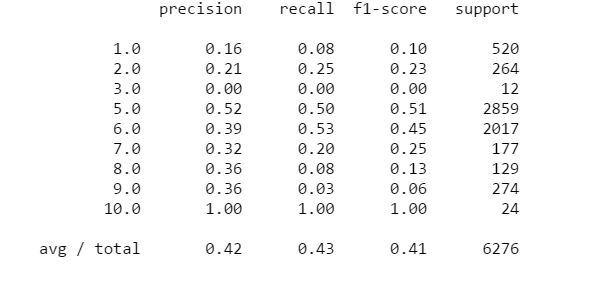
\includegraphics[height=2.5in, width=3.2in]{RandomForest}
\caption{Random Forest}
\end{figure}

Random Forest algorithm implementation resulted into accuracy of 43.04$\%$ and precision of 42$\%$ with F1 score of 41$\%$.

\subsubsection{Logistic Regression}
Logistic regression helps to explain the relationship between one dependent(binary form) and one or more independent variables for predictive analysis.

\begin{figure}[H]
\centering
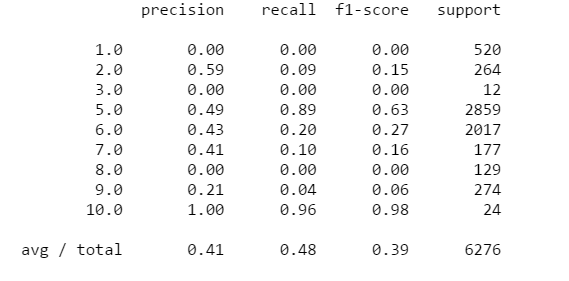
\includegraphics[height=2.5in, width=3.2in]{Logistic}
\caption{Logistic Regression}
\end{figure}

Logistic Regression gave overall better results amongst all algorithms accuracy of 48.18$\%$ and precision of 41$\%$ with F1 score of 39$\%$. 
Hence we will proceed with results obtained through Logistic Regression implementation. 

\subsection{Evaluation Strategies And Inference}
The F1 score (also F-score or F-measure) is a measure of a test accuracy. It considers both the precision and the recall of the test to compute the score: precision is the number of correct positive results divided by the number of all positive results, and recall is the number of correct positive results divided by the number of positive results that should have been returned. The F1 score can be interpreted as a weighted average of the precision and recall, where an F1 score reaches its best value at 1 and worst at 0.

The Vehicle models from different manufacturers were analysed and compared over the feature variables such as fuel consumption, $CO_{2}$ emission,Annual Fuel Cost as per usage, performance based on various driving conditions etc. A score between 1-10, with 10 being Cleanest Performance Vehicle.
The rating reflects vehicle tailpipe emissions that contribute to local and regional air pollution, creating problems such as smog, haze, and health issues. 

Before a new vehicle model can be sold, sample vehicles are tested under tightly controlled conditions. Their tailpipe emissions are captured and measured using sophisticated monitoring techniques. The results determine the emission standard that the vehicle meets.

Emission standards are for the major pollutants in vehicle exhaust:
1) NMOG, NMHC, or THC-types of carbon-containing compounds, including hydrocarbons \\
2) $NO_{x}$-Oxides of Nitrogen, which combine with hydrocarbons to create smog 
PM-Particulate Matter, tiny particles of solid matter that lodge in the lungs and deposit on buildings \\ 
3) CO-Carbon Monoxide, a colorless, odorless, poisonous gas \\
4) HCHO-Formaldehyde, a lung irritant and carcinogen 

Results for the predictive analysis scores obtained using Logistic Model were used for further data visualization. 

\section{Data Visualization}
\subsection{Pre-Analysis Data Plots}

Preliminary analysis was performed on the data set in R and Python to plot graphs to understand the fuel efficiency and carbon emission by selected car models as shown in the graphs below.

The 2 plots shown below compare highest and lowest carbon emissions(grams per miles) by cars based on brands(Fiat, Honda, Mini, Rolls Royce etc).

\begin{figure}[H]
\centering
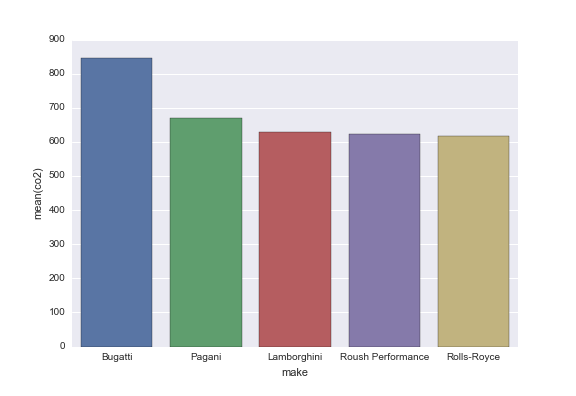
\includegraphics[height=2.2in, width=3.2in]{highco2}
\caption{Highest level of CO2 Emissions by different Car Brands}
\end{figure}

\begin{figure}[H]
\centering
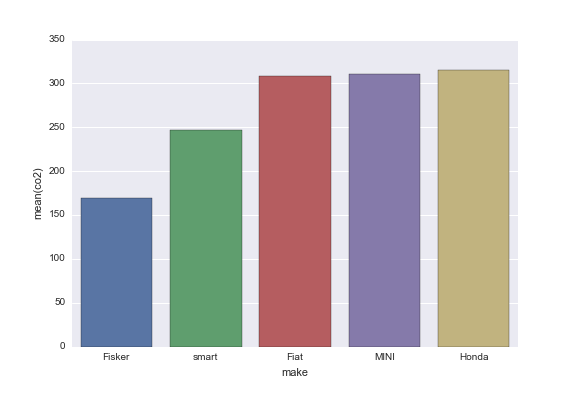
\includegraphics[height=2.2in, width=3.2in]{lowco2}
\caption{Lowest level of CO2 Emissions by different Car Brands}
\end{figure}

The graph below compares the carbon emission contributed by each fuel type annually over the period 1975-2016.

\begin{figure}[H]
\centering
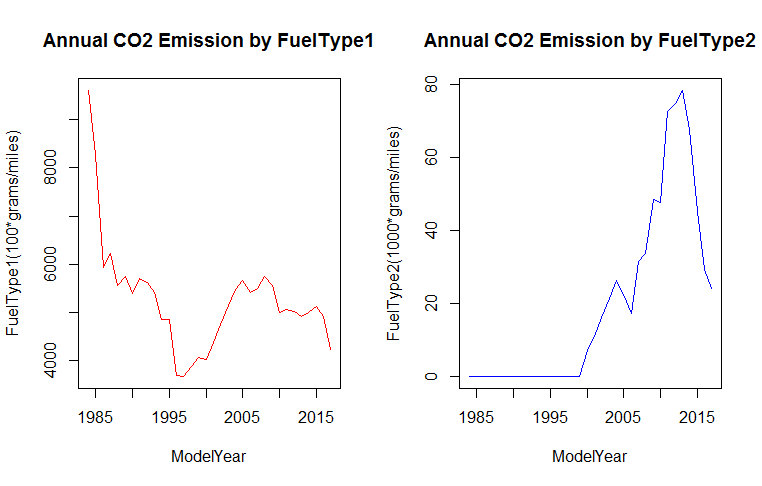
\includegraphics[height=2.7in, width=3.2in]{FT1VSFT2}
\caption{Annual Carbon Emission based on Fuel Type}
\end{figure}

\subsection{Predictive Analysis Plots}
Interactive Graphs, Pie-charts, plots and various other visualization techniques were implemented to observe the data and analyse behaviour of feature variables. 

\textbf{Distribution in Logistic Model}

The overall score distribution over total car production by Logistic Model is depicted using Bar Graph.

\begin{figure}[H]
\centering
\includegraphics[height=3in, width=3.3in]{ScoreDistribution}
\caption{Score VS No. Of Vehicles}
\end{figure}

\textbf{Fuel Economy VS Carbon Emission}

The line graphs below show the Fuel Economy and $CO_2$ over the period of time. The two curves are essentially inversely proportional to each other, i.e., vehicle tailpipe $CO_{2}$ 
emissions (grams per mile) are proportional to fuel consumption (gallons per mile), which is the reciprocal of fuel economy (miles per gallon). 

\begin{figure}[H]
\centering
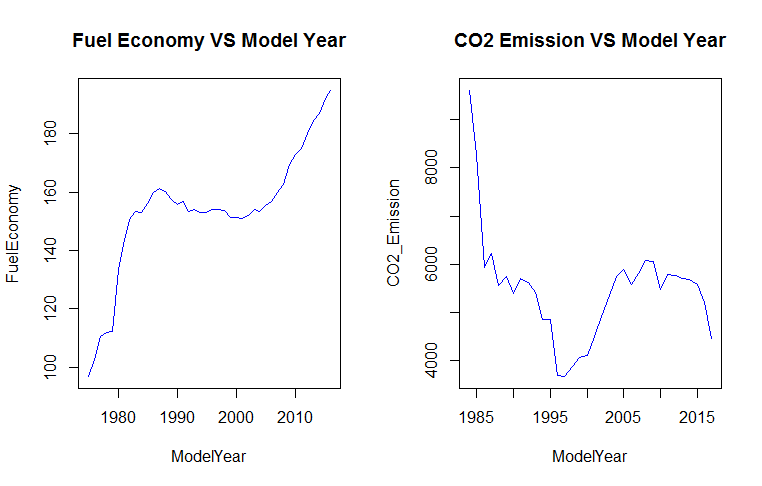
\includegraphics[height=3in, width=3.3in]{FuelEcoVSCO2Emission}
\caption{Fuel Economy VS CO2 Emission}
\end{figure}

\textbf{Carbon Emission by Various Make Vehicles}
Bubble Plot was implemented using D3js in Python to understand the overall $CO_{2}$ emitted by vehicles over the period of 1975-2017 based on their manufacturer. The bubble size denote the amount of $CO_2$ emitted by each make. Additionally, the plot helps to understand which make vehicles dominate the consumer industry. 

\begin{figure}[H]
\centering
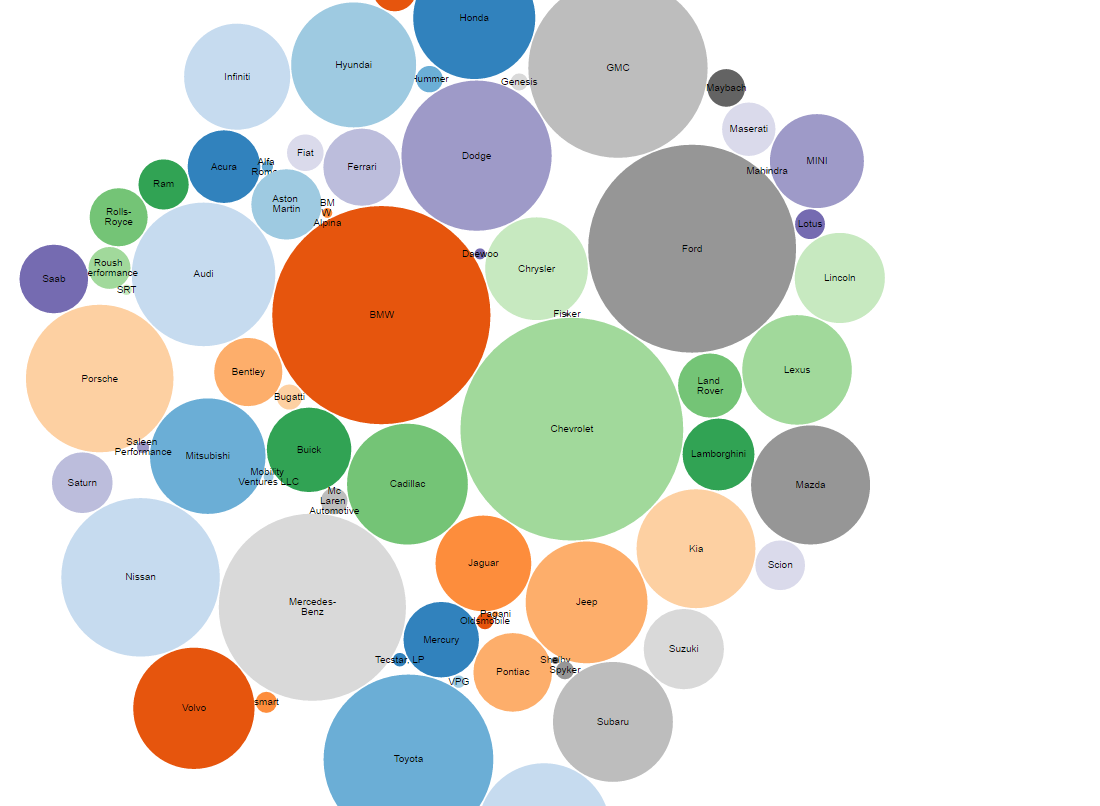
\includegraphics[height=3in, width=3.5in]{makeVSco2}
\caption{Manufacturers vs CO2 Emission}
\end{figure}

\textbf{Carbon Emission by Different Types of Fuels}

\begin{figure}[H]
\centering
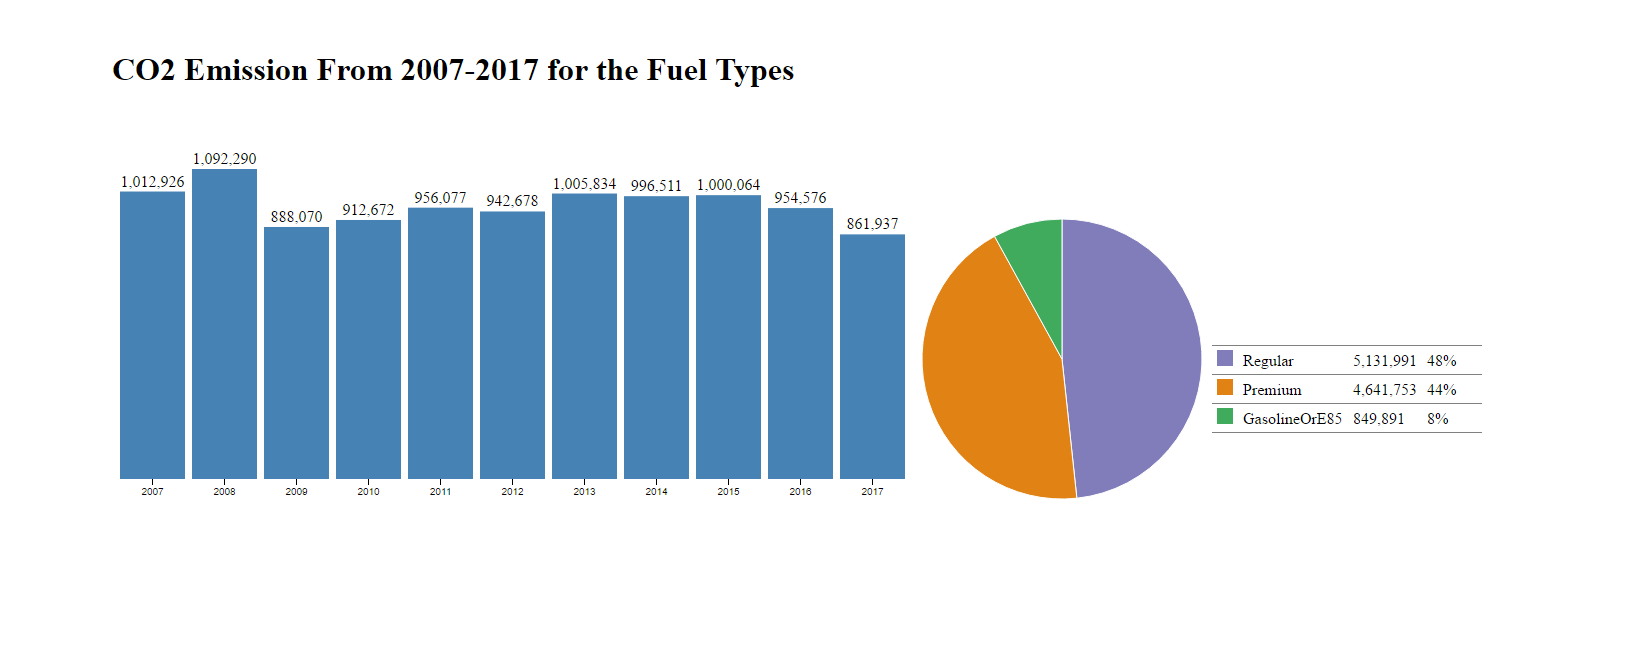
\includegraphics[height=2.8in, width=3.5in]{co2VSfueltyp1}
\caption{(a):FuelType vs CO2 Emission}
\end{figure}


The bar graph in Figure-a shows total $CO_{2}$ emitted from 2007 to 2017 while the pie-chart depicts the distribution of total carbon emission based on fuel type.

\begin{figure}[H]
\centering
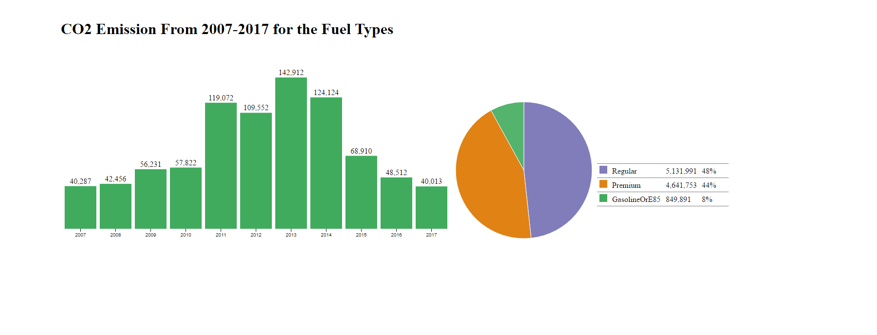
\includegraphics[height=2.8in, width=3.9in]{co2VSfueltyp2}
\caption{(b):FuelType vs CO2 Emission}
\end{figure}

The above figure shows bar graph with $CO_{2}$ emitted by usage of Gasoline fuel from the 2007 to 2017. 

\textbf{Carbon Emission based on Drive Type}
This graph shows the amount of $CO_{2}$ emitted by vehicles based on their drive types annually. 

\begin{figure}[H]
\centering
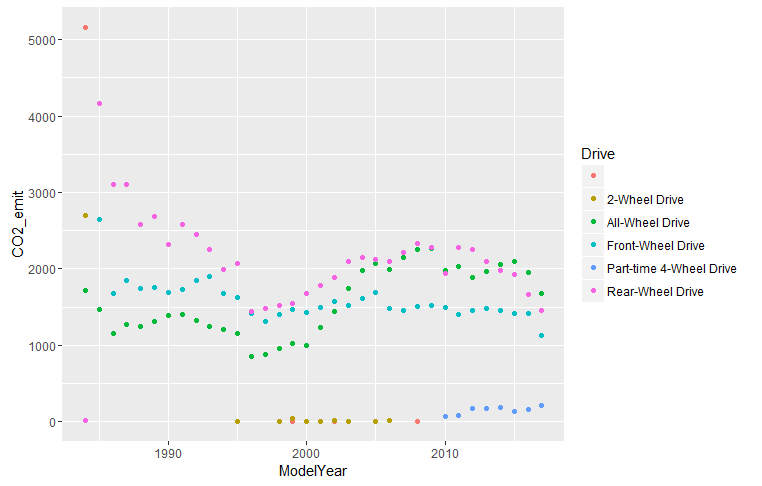
\includegraphics[height=3in, width=3.5in]{DriveCO2}
\caption{Model Year vs CO2 Emission w.r.t Drive Type}
\end{figure}

\textbf{Vehicle Acceleration}
This graph shows performance of each vehicle namely car,truck,SUV etc. over the course of time.

\begin{figure}[H]
\centering
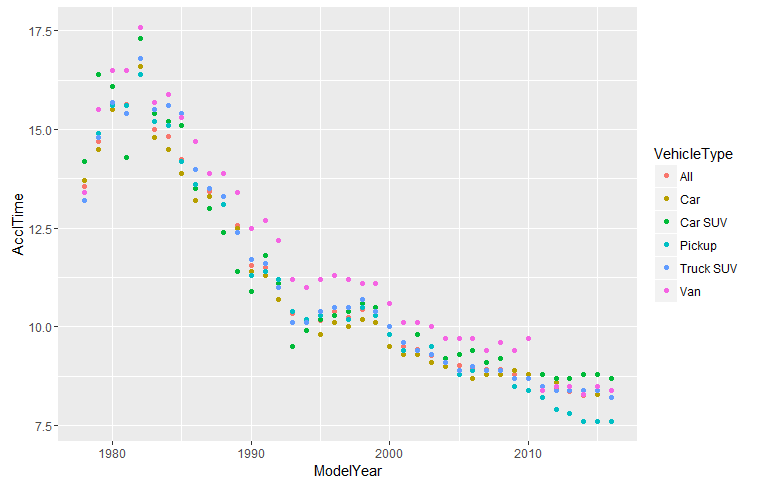
\includegraphics[height=3in, width=3.5in]{acclVStyp}
\caption{Acceleration VS Model Year w.r.t VehicleType}
\end{figure}

Although vehicle performance can be evaluated in many ways, including vehicle handling, braking, and acceleration. In the context of this project, acceleration is an important metric because there is a general correlation between how quickly a vehicle can accelerate and fuel economy. Since the early 1980s, there has been a clear downward trend in 0-to-60 times. The graph shows the average new vehicle 0-to-60 acceleration time from MY 1978 to MY 2016. The average new vehicle in MY 2016 is projected to have a 0-to-60 time of approx. 8 seconds, which is the fastest average 0-to-60 time since the database began in 1975. 

\begin{figure}[H]
\centering
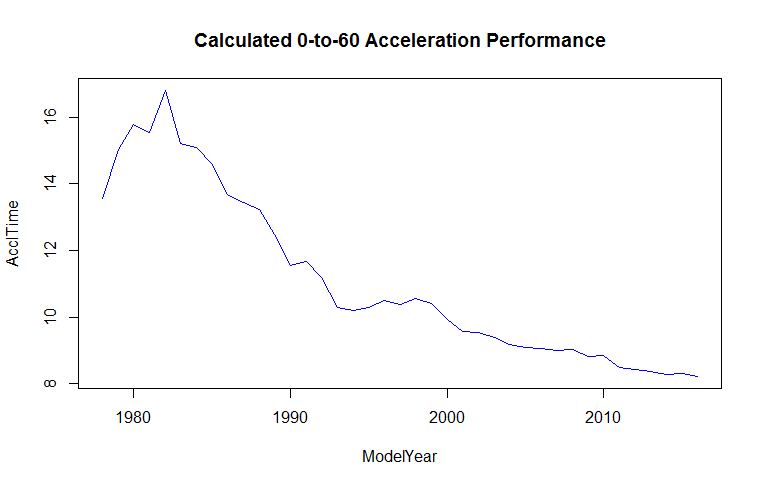
\includegraphics[height=3in, width=3.5in]{AcclPerf}
\caption{Acceleration VS Model Year}
\end{figure}

\textbf{Annual Vehicle Production based on Types}
\begin{figure}[H]
\centering
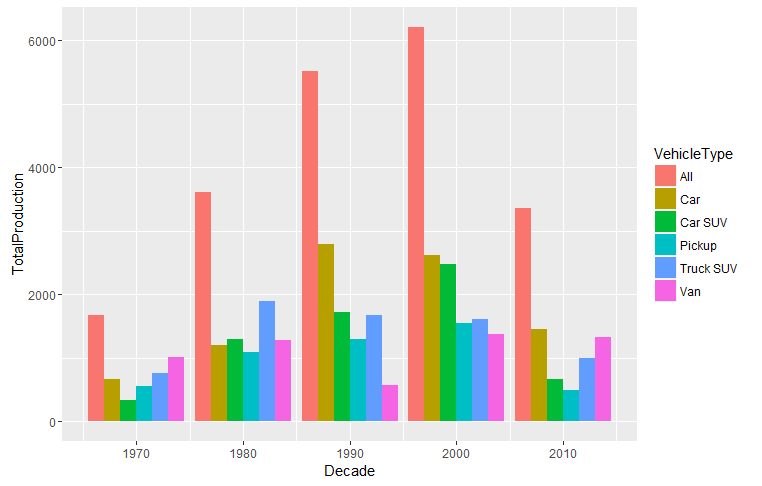
\includegraphics[height=2.7in, width=3.5in]{vehicleOptn}
\caption{TotalProduction VS Decade w.r.t VehicleType}
\end{figure}

The aforementioned dodged barplot shows Total Vehicle Production based on different types of Vehicles over a decade from 1975-2017. And a barplot below shows the changes in Fuel Efficiency(in MileperGallon) of each vehicle type over every decade from 1975-2016.

\begin{figure}[H]
\centering
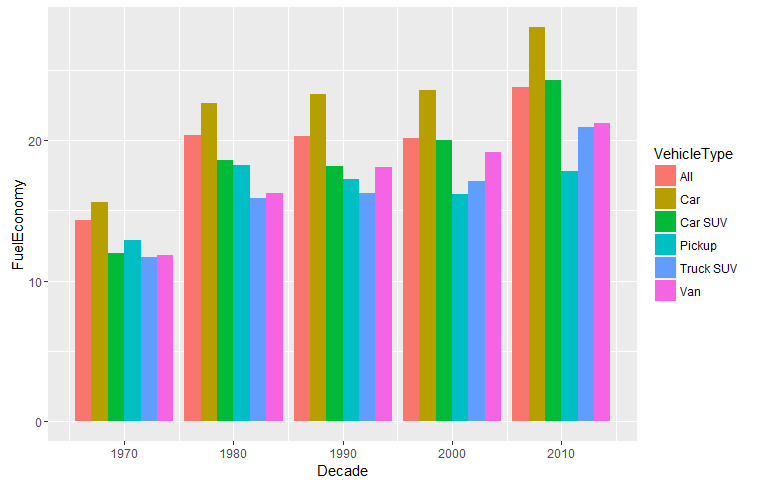
\includegraphics[height=2.7in, width=3.5in]{FuelEcoVTyp}
\caption{FuelEconomy VS Decade w.r.t VehicleType}
\end{figure}

\section{Corrective Measures / Solutions}
\begin{itemize}

    \item Using Clean vehicles with score of 7 or above can help increase fuel economy and reduce carbon emission.
    
    \item To reduce overall $CO_{2}$ emission due to usage of vehicles, we need to start using more fuel efficient vehicles. Since the $CO_{2}$ emission in inversely proportional to Fuel Efficiency (as seen in Figure:11).
    
    Figures: 17 and 18 show that recent years, manufactures have made available, more choices of vehicles with higher fuel economy to the consumers, thus lower tailpipe CO2 emissions compared to early years. These choices reflect both a more diverse range of technology packages on conventional gasoline and diesel vehicles as well as an increasing number of alternative fuel vehicle offerings. But comparatively the production of rest of the vehicles should also be reduced to see notable decrease in the carbon emissions.
    
    \item All five vehicle types have steadily increased fuel economy in recent years and are at or near their record high fuel economy as seen in Figure:18. However, the market shift towards SUVs in recent years(Figure:17) has offset some of the benefits that otherwise would have been achieved due to the increased fuel economy within each vehicle type.
    
    \item Horsepower (HP) is a direct measure of vehicle power. In the past, higher horse-power generally increased $CO_{2}$ emissions and decreased fuel economy. In recent years, new engine technologies like turbo and hybrid engines have significantly lowered the inverse proportionality. Thus, the engine make in the vehicles should be modified with these recent technologies to reduce the harmful gas emission. 
    
    \item As seen in Figure 15: Part-Time 4 Wheel Drive shows significant drop in carbon emission compared to 2WD and 4WD vehicles. Part-time 4-Wheel Drive is basically has 2 wheel drive as main mode for everyday pavement use and operates  only on rear wheels and when 4WD is engaged front wheels are powered as well.\cite{Walczak} This helps reduce the power and fuel consumption. Thus, Part-time 4 wheel drive technology can also help achieve the goal.    
    
    \item Alternative fuel resources should be taken into consideration like solar-power vehicles or vehicles that operate on electricity. Car-pooling , taking cycles or walking to nearby places will also reduce the vehicle usage thereby reducing fuel consumption and $CO_{2}$ emission. 
    
    \item Vehicle acceleration is determined by many factors, including weight, horsepower, transmission type, engine type, and body style. Most of the these factors that affect acceleration also influence vehicle fuel economy as seen in aforementioned plots(Figures:16 and 17). Thus is can be said that there exists a correlation between faster 0-to-60 times and lower fuel economy. Therefore, irrespective of other factors, a vehicle with more power will likely have faster 0-to-60 acceleration and lower fuel economy.
    
\end{itemize}

\section{Conclusion}

This report provides a reference for $CO_{2}$ emission,fuel economy and latest technology trends for personal vehicles in United States. The data supporting this report was obtained from the U.S.Environment Protection Agency. 

The project identified highest and lowest $CO_{2}$ emitting vehicle manufacturers. Levels of $CO_{2}$ emission were calculated and compared with various feature variables such as \begin{itemize}
    \item Vehicle Type(Eg. Car,SUV,Trucks) 
    \item Drive Type (Eg. 2WD,4WD,Part-time 4WD) 
    \item Fuel Type (Eg. Regular,Premium,Gasoline)
\end{itemize}
It was also seen that HP and Weight of the vehicle contributed to the carbon emission. Improving the acceleration of vehicle will also result into better fuel efficiency. 

Thus implementing suggestions provided from observing the trends in the dataset significant change can be brought into the environment thereby contributing to sustaining ecological balance around the world.

\section{Acknoledgements}

We would like to express our sincere gratitude to Prof. Gregor von Laszewski and the course AI's, Prashanth Balasubramani and Jerome Mitchell for their constant guidance and suggestions throughout the project completion process. 

\bibliographystyle{IEEEtran}
\bibliography{references}

\end{document}
